\documentclass[11pt]{cernrep}
\usepackage{graphicx,epsfig}
\bibliographystyle{lesHouches}


% Packages needed for this section
\usepackage{amsmath}
\usepackage{hepunits}
\usepackage[caption=false]{subfig}
\usepackage[utf8]{inputenc}

% Comments to be commented out when done
\usepackage{color}
\definecolor{darkgreen}{rgb}{0,0.5,0}
\newcommand{\jdt}[1]{\textbf{\textcolor{darkgreen}{(#1 --jdt)}}}
\definecolor{darkblue}{rgb}{0,0,0.5}
\newcommand{\gs}[1]{\textbf{\textcolor{darkblue}{(#1 --gs)}}}

\begin{document}

\section{SYSTEMATICS OF QUARK/GLUON TAGGING\protect\footnote{Section coordinators: Gregory Soyez and Jesse Thaler}$^{,}$\protect\footnote{Contributing authors: Marat Freytsis, Philippe Gras, Deepak Kar, Simon Pl\"atzer, Andrzej Siodmok, Peter Skands, and Davison Soper}$^{,}$\protect\footnote{Additional input: Samuel Bein, Andy Buckley, Jon Butterworth, Mario Campanelli, Andrew Larkoski, Peter Loch, Zoltan Nagy, Chris Pollard, Salvatore Rappoccio, Alexander Schmidt, Frank Tackmann, and Wouter Waalewijn}}

By measuring the substructure of a jet, one can assign it a ``quark'' or ``gluon'' tag.  In the eikonal limit, quark/gluon discrimination is determined solely by the color factor of the initiating parton ($C_F$ versus $C_A$).  In this section, we confront the challenges faced when going beyond this leading-order understanding, using parton shower generators to assess the impact of higher-order perturbative and non-perturbative physics.  Working in the idealized context of electron-positron collisions, where there exists an unambiguous definition of quark and gluon jets, we find a fascinating interplay between perturbative shower effects and non-perturbative hadronization effects.

\subsection{Overview}
\label{quarkgluon_sec:overview}

Jets are a robust tool for studying short-distance collisions involving quarks and gluons.  With a suitable jet definition, one can connect jet measurements made on clusters of hadrons to perturbative calculations made on clusters of partons.  More ambitiously, one can try to tag jets with a suitably-defined flavor label, thereby enhancing the fraction of, say, quark-tagged jets over gluon-tagged jets.  This is relevant for searches for physics beyond the standard model, where signals of interest are often dominated by quarks while the corresponding backgrounds are dominated by gluons.  A wide variety of quark/gluon discriminants have been proposed \cite{Gallicchio:2011xq,Gallicchio:2012ez,Krohn:2012fg,Pandolfi:1480598,Chatrchyan:2012sn,Larkoski:2013eya,Larkoski:2014pca}, and there is a growing catalog of quark/gluon studies at the Large Hadron Collider (LHC) \cite{Aad:2014gea,Aad:2014bia,Khachatryan:2014dea,Aad:2015owa,Khachatryan:2015bnx,Aad:2016oit}.

In order to achieve robust quark/gluon tagging, though, one needs theoretical and experimental control over quark/gluon radiation patterns.  At the level of eikonal partons, a quark radiates proportional to its $C_F = 4/3$ color factor while a gluon radiates proportional to $C_A = 3$.  In this section, we demonstrate that quark/gluon discrimination performance is highly sensitive to subleading perturbative effects beyond the eikonal limit, such as $g \to q \overline{q}$ splittings and color coherence, as well as to non-perturbative effects such as color reconnection and hadronization.   While these effects are modeled (to differing degrees) in parton shower generators, they are relatively unconstrained by existing collider measurements, especially in the gluon channel.  The goal of this section is to highlight these uncertainties, which then suggests a set of future LHC measurements that will improve the modeling of jets in general and quark/gluon tagging in particular.

A common misconception about quark/gluon tagging is that it is an intrinsically ill-defined problem.  Of course, quark and gluon partons carry color while jets are composed of color-singlet hadrons, so the labels ``quark'' and ``gluon'' are fundamentally ambiguous.  But this is philosophically no different from the fact that a ``jet'' is fundamentally ambiguous and one must therefore always specify a concrete jet finding procedure.  As discussed in Sec.~\ref{quarkgluon_sec:def}, the proper way to think about quark/gluon discrimination is in the context of unambiguous hadron-level measurements.  In that sense, quark/gluon tagging is a well-defined technique for enhancing desired signals over undesired backgrounds.

There are a wide range of possible quark/gluon discriminants and a similarly large range of ways to quantify discrimination power.  As a concrete set of discriminants, we consider the generalized angularities $\lambda_\beta^\kappa$ \cite{Larkoski:2014pca} (see also \cite{Berger:2003iw,Almeida:2008yp,Ellis:2010rwa,Larkoski:2014uqa}).  As discussed further in Sec.~\ref{quarkgluon_sec:genang}, we consider five different $(\kappa, \beta)$ working points, which roughly map onto five variables in common use in the literature:
\begin{equation}
\text{multiplicity}, \quad p_T^D, \quad \text{LHA}, \quad \text{width} 
, \quad \text{mass} .
\end{equation}
Here, multiplicity is the hadron multiplicity within the jet, $p_T^D$ was defined in Refs.~\cite{Pandolfi:1480598,Chatrchyan:2012sn}, LHA refers to the ``Les Houches Angularity'' (named after the venue of this workshop), width is closely related to jet broadening \cite{Catani:1992jc,Rakow:1981qn,Ellis:1986ig}, and mass is closely related to jet thrust \cite{Farhi:1977sg}.  To quantify discrimination performance, we focus on classifier separation (a default output of TMVA \cite{2007physics...3039H}):
\begin{equation}
\Delta =  \frac{1}{2} \int \text{d} \lambda \, \frac{\bigl(p_q(\lambda) - p_g(\lambda)\bigr)^2}{p_q(\lambda) + p_g(\lambda)},
\end{equation}
where $p_q$ ($p_g$) is the probability distribution for a quark-tagged (gluon-tagged) sample.  Other potential performance metrics are discussed in Sec.~\ref{quarkgluon_sec:classsep}.

We begin our parton shower generator predictions for quark/gluon discrimination in Sec.~\ref{quarkgluon_sec:ee}, using an idealized setup with $e^+e^-$ collisions.  Here, we can use the following processes as unambiguous proxies for quark and gluon jets:
\begin{align}
\text{``quark jets''}: \quad & e^+e^- \to (\gamma/Z)^* \to u \overline{u}, \\
\text{``gluon jets''}: \quad & e^+e^- \to h^* \to g g,
\end{align}
where $h$ is the Higgs boson.  These processes are physically distinguishable by the quantum numbers of the associated color singlet production operator, giving a way to label quarks and gluons without reference to the final state.  We compare four different parton shower generators both before hadronization (``parton level'') and after hadronization (``hadron level''):
\begin{itemize}
\item \textsc{Pythia 8.205} \cite{Sjostrand:2014zea},
\item \textsc{Vincia 1.201} \cite{Giele:2013ema},
\item \textsc{Herwig++ 2.7.1} \cite{Bellm:2013hwb},
\item \textsc{Sherpa 2.1.1} \cite{Gleisberg:2008ta}.
\end{itemize}
We also show parton-only results for a new generator:
\begin{itemize}
\item \textsc{Deductor 1.0.2} \cite{Nagy:2014mqa}.
\end{itemize}
In the future, we plan to make \textsc{Dire} \cite{Hoche:2015sya} predictions about quark/gluon discrimination as well as investigate predictions from analytic resummation \cite{Larkoski:2013eya,Larkoski:2014pca}.

As we will see, the differences between these generators arise from physics at the interface between perturbative showering and non-perturbative fragmentation.  One might think that the largest differences between generators would appear for infrared-and-collinear (IRC) unsafe observables like multiplicity and $p_T^D$, where non-perturbative hadronization plays an important role.  Surprisingly, comparably-sized differences are also seen for the IRC safe angularities, indicating that these generators have different behavior even at the level of the perturbative final state shower.  In Sec.~\ref{quarkgluon_sec:ee_scales}, we study these differences as a function of collisions energy $Q$, jet radius $R$, and strong coupling constant $\alpha_s$, showing that the generators have somewhat different discrimination trends.  In Sec.~\ref{quarkgluon_sec:ee_settings}, we compare the default parton shower configurations to physically-motivated changes, showing that modest changes to the shower/hadronization parameters can give rather large differences in quark/gluon separation power.

At the end of the day, most of the disagreement between generators is due to gluon radiation patterns.  This is not so surprising, since all of the generators have been tuned to reproduce distributions from $e^+ e^-$ colliders, and quark (but less so gluon) radiation patterns are highly constrained by event shape measurements at LEP \cite{Heister:2003aj,Abdallah:2003xz,Achard:2004sv,Abbiendi:2004qz}.  In Sec.~\ref{quarkgluon_sec:pp}, we suggest a possible analysis strategy at the LHC to specifically constrain gluon radiation patterns.  At a hadron collider, the distinction between quark jets and gluon jets is rather subtle, since radiation patterns depend on color connections between the measured final state jets and the unmeasured initial state partons.  That said, we suspect that much can be learned from hadron-level measurements, even without isolating ``pure'' quark or gluon samples.

We present our final recommendations and conclusions in Sec.~\ref{quarkgluon_sec:conclude}.  The main take home message from this study is that, contrary to the standard lore, measurements at $e^+e^-$ colliders are insufficient to constrain uncertainties in the final state shower.   Therefore, gluon-enriched measurements at the LHC will be crucial to achieve robust quark/gluon discrimination.

\subsection{What is a Quark/Gluon Jet?}
\label{quarkgluon_sec:def}

As part of the 2015 Les Houches workshop, an attempt was made to define exactly what is meant by a ``quark jet'' or ``gluon jet''.  Here are some suggested options for defining a quark jet, in order from most ill-defined to most well-defined.  Related statement can be made for gluon jets.

\noindent \textbf{A quark jet is...}
\begin{itemize}
\item \textbf{A quark parton.}  This definition (incorrectly) assumes that there is a one-to-one map between a jet and its initiating parton.  Because it neglects the important role of additional radiation in determining the structure of a jet, we immediately dismiss this definition.
\item \textbf{A Born-level quark parton.}  This definition at least acknowledges the importance of radiative corrections to jet production, but it leaves open the question of how exactly to define the underlying Born-level process from an observed final state.  (For one answer valid at the parton level, see flavored jet algorithms below.)
\item \textbf{An initiating quark parton in a final state parton shower.}  We suspect that this is the definition most LHC experimentalists have in mind.  This is sometimes referred to as the ``max-$p_T$'' prescription (see further discussion in \cite{Buckley:2015gua}), though it assumes that the parton shower history is meaningful, which may not be the case beyond the strongly-ordered or leading-logarithmic approximations.  Because the parton shower is semi-classical, this definition neglects the impact of genuinely quantum radiative corrections as well as non-perturbative hadronization. 
\item \textbf{An eikonal line with baryon number 1/3 and carrying triplet color charge.}  This is another semi-classical definition that attempts to use a well-defined limit of QCD to define quarks in terms of light-like Wilson lines.  Philosophically, this is similar to the parton shower picture, with a similar concern about how to extrapolate this definition away from the strict eikonal limit.
\item \textbf{A parton-level jet object that has been quark-tagged using an IRC safe flavored jet algorithm.}  This is the strategy adopted in \cite{Banfi:2006hf}.  While this definition neglects the impact of hadronization, it does allow for the calculation of quark jet cross sections at all perturbative orders, including quantum corrections.
\end{itemize}
The unifying theme in the above definitions is that they try to identify a quark as an object unto itself, without reference to the specific final state of interest.  However, it is well-known that a ``quark'' in one process may not look like a ``quark'' in other process, due to color correlations with the rest of the event, especially the initial state in $pp$ collisions.  The next definition attempts to deal with the process dependence in defining quarks. 
\begin{itemize}
\item \textbf{A quark operator appearing in a hard matrix element in the context of a factorization theorem.}  This is similar to the attitude taken in \cite{Gallicchio:2011xc}.  In the context of a well-defined cross section measurement, one can (sometimes) go to a limit of phase space where the hard production of short-distance quarks and gluons factorizes from the subsequent long-distance fragmentation.  This yields a nice (gauge-covariant) operator definition of a quark jet.  That said, even if a factorization theorem does exist for the measurement of interest, this definition is potentially ambiguous beyond leading power.
\end{itemize}
The definition we adopt for this study is inspired by the idea that one should think about quark/gluon tagging in the context of a specific measurement, but it tries to avoid relying on the presence of a factorization theorem.
\begin{itemize}
\item \textbf{A phase space region (as defined by an unambiguous hadronic fiducial cross section measurement) that yields an enriched sample of quarks (as interpreted by some suitable, though fundamentally ambiguous, criterion).}  Here, the goal is to \emph{tag} a phase space region as being quark-like, rather than try to determine a truth definition of a quark.  This definition has the advantage of being explicitly tied to hadronic final states and to the discriminant variables of interest.   Of course, the main challenge with this definition is how to determine the criterion that corresponds to successful quark enrichment.  For that, we will have to rely to some degree on the other less well-defined notions of what a quark jet is.
\end{itemize}  

It is worth emphasizing that this last definition separates the measurement process from the interpretation process.  That is, one first measures hadron-level discriminant variables on a final state of interest, and only later does one interpret exactly what that discrimination accomplishes (either as quark/gluon separation or as some more sophisticated classification).  In Sec.~\ref{quarkgluon_sec:conclude}, we will recommend that the LHC experiments perform measurements of the generalized angularities $\lambda_\beta^\kappa$ in well-defined hadron-level final states; it is then a separate interpretation step to infer something about parton-level quark/gluon radiation patterns from these hadron-level measurements.

\subsection{Generalized Angularities}
\label{quarkgluon_sec:genang}

\begin{figure}
\centering
\subfloat{
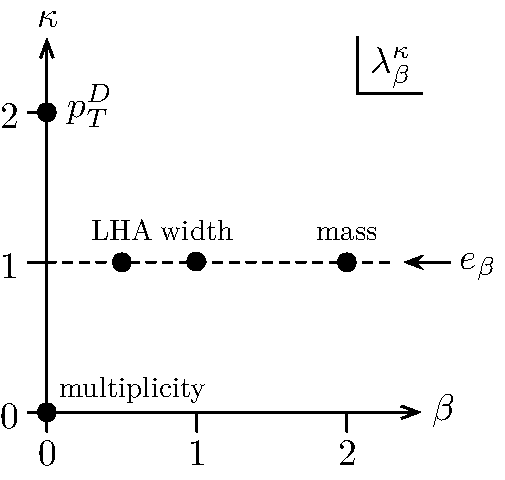
\includegraphics[scale = 0.7]{quarkgluon_fig_lambda_space.pdf}
}
\caption{Two parameter family of generalized angularities, adapted from \cite{Larkoski:2014pca}.  The dots correspond to the five benchmark angularities used in thiss study.  The horizontal line at $\kappa = 1$ corresponds to the IRC safe angularities.}
\label{quarkgluon_fig:lambda_space}
\end{figure}

A wide variety of quark/gluon discriminants have been proposed (see \cite{Gallicchio:2012ez} for an extensive catalog), but here we limit ourselves to a two-parameter family of generalized angularities \cite{Larkoski:2014pca}, shown in Fig.~\ref{quarkgluon_fig:lambda_space}.  These are defined as
\begin{equation}
\label{quarkgluon_eq:genang}
\lambda^{\kappa}_{\beta} = \sum_{i \in \text{jet}} z_i^\kappa \theta_i^\beta,
\end{equation}
where $i$ runs over the jet constituents, $z_i \in [0,1]$ is a momentum fraction, and $\theta_i \in [0,1]$ is a (normalized) angle to the jet axis.  The parameters $\kappa \ge 0$ and $\beta \ge 0$ determine the momentum and angle weighting, respectively.  For $\kappa = 1$, the generalized angularities are IRC safe and hence calculable in perturbation theory \cite{Larkoski:2014uqa} (see also \cite{Ellis:2010rwa,Larkoski:2013paa,Larkoski:2014tva,Procura:2014cba,Hornig:2016ahz}).  For general $\kappa \not= 1$, there are quasi-perturbative techniques based on generalized fragmentation functions \cite{Larkoski:2014pca} (see also \cite{Krohn:2012fg,Waalewijn:2012sv,Chang:2013rca,Chang:2013iba}).  In our parton shower studies, we determine $\lambda^{\kappa}_{\beta}$ using all constituents of a jet, though one could also consider using charged-particle-only angularities to improve robustness to pileup.

For our $e^+ e^-$ study, we cluster jets using the $ee$-variant of the anti-$k_t$ algorithm \cite{Cacciari:2008gp}, with $|\vec{p}|$-ordered winner-take-all recombination \cite{Larkoski:2014uqa,Bertolini:2013iqa,Salam:WTAUnpublished} to determine the jet axis $\hat{n}$.  Unlike standard $E$-scheme recombination \cite{Blazey:2000qt}, the winner-take-all scheme yields a jet axis $\hat{n}$ that does not necessarily align with the jet momentum $\vec{p}$; this turns out to be a desirable feature for avoiding soft recoil effects \cite{Larkoski:2013eya,Larkoski:2014uqa,Catani:1992jc,Dokshitzer:1998kz,Banfi:2004yd}.  We define
\begin{equation}
z_i \equiv \frac{E_i}{E_{\rm jet}}, \qquad \theta_i \equiv \frac{\Omega_{i \hat{n}}}{R},
\end{equation}
where $\Omega_{i \hat{n}}$ is the opening angle to the jet axis and $R$ is the jet radius (taken to be $R = 0.6$ by default).  To translate our $ee$ study to an eventual $pp$ study (left to future work), one would use the standard $pp$ version of anti-$k_t$ with $p_T$-ordered winner-take-all recombination, defining
\begin{equation}
z_i \equiv \frac{p_{Ti}}{\sum_{j \in \text{jet}} p_{Tj}}, \qquad \theta_i \equiv \frac{R_{i \hat{n}}}{R},
\end{equation}
where $R_{i \hat{n}}$ is the rapidity-azimuth distance to the jet axis.



By adjusting $\kappa$ and $\beta$, one can probe different aspects of the jet fragmentation.  We consider five benchmark values for $(\kappa, \beta)$ indicated by the black dots in Fig.~\ref{quarkgluon_fig:lambda_space}:
\begin{equation}
\label{quarkgluon_eq:benchmarkang}
\begin{aligned}
(0,0) &= \text{hadron multiplicity},\\
(2,0) &\Rightarrow p_T^D \text{  \cite{Pandolfi:1480598,Chatrchyan:2012sn} (specifically $\lambda^{2}_{0} = (p_T^D)^2$)},\\
(1,0.5) & = \text{Les Houches Angularity (LHA)},\\
(1,1) &= \text{width or broadening \cite{Catani:1992jc,Rakow:1981qn,Ellis:1986ig}},\\
(1,2) & \Rightarrow \text{mass or thrust \cite{Farhi:1977sg} (specifically $\lambda^{1}_{2} \simeq m_{\rm jet}^2 / E_{\rm jet}$)}.
\end{aligned}
\end{equation}
Except for the LHA, these angularities (or their close cousins) have already been used in quark/gluon discrimination studies.  The LHA has been included to have an IRC safe angularity that weights energies more heavily than angles, similar in spirit to the $\beta = 0.2$ value advocated in ref.~\cite{Larkoski:2013eya}.

For the IRC safe case of $\kappa = 1$, there is an alternative version
of the angularities based on energy correlation functions \cite{Larkoski:2013eya} (see also \cite{Banfi:2004yd,Jankowiak:2011qa}
\begin{equation}
\text{ecf}_\beta = \sum_{i < j \in \text{jet}} z_i z_j \theta_{ij}^\beta \simeq \lambda^{1}_{\beta},
\end{equation}
where equality holds in the extreme eikonal limit.\footnote{This equality also relies on using a recoil-free axis choice $\hat{n}$ to define $\theta_i$.  Amusingly, $\lim_{\beta \to 0} \text{ecf}_\beta = (1 - \lambda^{2}_{0})/2$ (i.e.~$\kappa = 2$, $\beta = 0$), such that the $\beta \to 0$ limit of the IRC safe energy correlation functions corresponds to the IRC unsafe $p_T^D$.}  For the $e^+ e^-$ case, the pairwise angle $\theta_{ij}$ is typically normalized to the jet radius as $\theta_{ij} \equiv \Omega_{ij}/R$.   To avoid a proliferation of curves, we will not show any results for $\text{ecf}_\beta$.  We will also neglect quark/gluon discriminants that take into account azimuthal asymmetries within the jet, though observables like the covariance tensor \cite{Gallicchio:2012ez} and 2-subjettiness \cite{Thaler:2010tr,Thaler:2011gf} can improve quark/gluon discrimination.

\subsection{Classifier Separation}
\label{quarkgluon_sec:classsep}

Since we will be testing many parton shower variants, we need a way to quantify quark/gluon separation power in a robust way that can easily be summarized by a single number.  For that purpose we use classifier separation,
\begin{equation}
\label{quarkgluon_eq:deltadef}
\Delta =  \frac{1}{2} \int \text{d} \lambda \, \frac{\bigl(p_q(\lambda) - p_g(\lambda)\bigr)^2}{p_q(\lambda) + p_g(\lambda)},
\end{equation}
where $p_q$ ($p_g$) is the probability distribution for the quark-tagged (gluon-tagged) sample as a function of the classifier $\lambda$.  Here, $\Delta = 0$ corresponds to no discrimination power and $\Delta = 1$ corresponds to perfect discrimination power.

A more common way to talk about discrimination power is in terms of receiver operating characteristic (ROC) curves.  At a point ($q$,$g$) on the ROC curve, where $q,g \in [0,1]$, one can define a selection that yields $q$ efficiency for quarks and $g$ mistag rate for gluons, or equivalently, a $(1-g)$ efficiency for gluons for a $(1-q)$ mistag rate for quarks.  To turn the ROC curve into a single number, it is common to report the gluon rejection rate at, say, 50\% quark efficiency.  Since we are more interested in understanding the relative performance between parton showers rather than the absolute performance, we will not show ROC curves here, though they can be easily derived from the $p_q$ and $p_g$ distributions.  If one observable has an everywhere better ROC curve than another (i.e.~it is Pareto optimal), then it will also have a larger $\Delta$ value.  The converse is not true, however, since depending on the desired working point, a ``bad'' discriminant as measured by $\Delta$ might still be ``good'' by another metric.  In that sense, $\Delta$ contains less information than the full ROC curve.

An alternative way to quantify discrimination power is through mutual information, which counts the number of ``bits'' of information gained from measuring a discriminant variable (see \cite{Larkoski:2014pca}).  Given a sample with quark fraction $f \in [0,1]$ and gluon fraction $(1-f)$, the mutual information with the truth (a.k.a. the truth overlap) is
\begin{equation}
I(T; \Lambda) = \int \text{d} \lambda \left(f \, p_q(\lambda) \log_2 \frac{p_q(\lambda)}{p_{\rm tot}(\lambda)} + (1-f) \, p_g(\lambda) \log_2 \frac{p_g(\lambda)}{p_{\rm tot}(\lambda)}   \right),
\end{equation}
where
\begin{equation}
p_{\rm tot}(\lambda) = f \, p_q(\lambda) + (1-f) \, p_g(\lambda).
\end{equation}
The choice $f = 1/2$ was used in Ref.~\cite{Larkoski:2014pca}, though other $f$ choices are plausible.  Though we will not use mutual information in this study, it is amusing to note that the second derivative of $I(T;\Lambda)$ with respect to $f$ is related to classifier separation as
\begin{equation}
\label{quarkgluon_eq:altdeltadef}
- \frac{\log 2}{4} \frac{\partial^2 I(T;\Lambda)}{\partial f^2} \Big|_{f = \frac{1}{2}} \equiv \Delta.
\end{equation}
One advantage of $\Delta$ over $I(T;\Lambda)$ is that the integrand in Eq.~\eqref{quarkgluon_eq:deltadef} is easier to plot and interpret, since it tracks the fractional difference between the signal and background at a given value of $\lambda$.\footnote{Another advantage of $\Delta$ over $I(T; \Lambda)$ arises when trying to assign statistical uncertainties to finite Monte Carlo samples.  Since $\Delta$ is defined as a simple integral, one can use standard error propagation to assign uncertainties to $\Delta$.  By contrast, because of the logarithms in $I(T; \Lambda)$, one has to be careful about a potential binning bias \cite{Larkoski:2014pca}.}

\subsection{Idealized Quark/Gluon Discrimination}
\label{quarkgluon_sec:ee}

To demonstrate the importance of final state evolution for quark/gluon discrimination, our studies are based on the idealized case of discriminating $e^+ e^- \to (\gamma/Z)^* \to u \bar{u}$ (quark-tagged) from $e^+ e^- \to h^* \to gg$ (gluon-tagged).  Here, the flavor of the outgoing jets is fixed by the Lorentz structure of the production vertex.  Of course, even in the quark-tagged sample, there can be ``gluon jets'', as in $e^+ e^- \to u \bar{u} g$ where a hard gluon recoils against a nearly collinear $u \bar{u}$.  This reflects the intrinsic ambiguity in defining jet flavor.   To resolve that ambiguity, we rely on the production vertex alone to define the truth-level jet flavor.  As our baseline, we operate at a center-of-mass collision energy of $Q = 200~\GeV$ with jet radius $R = 0.6$.  

\begin{figure}
\centering
\subfloat[]{
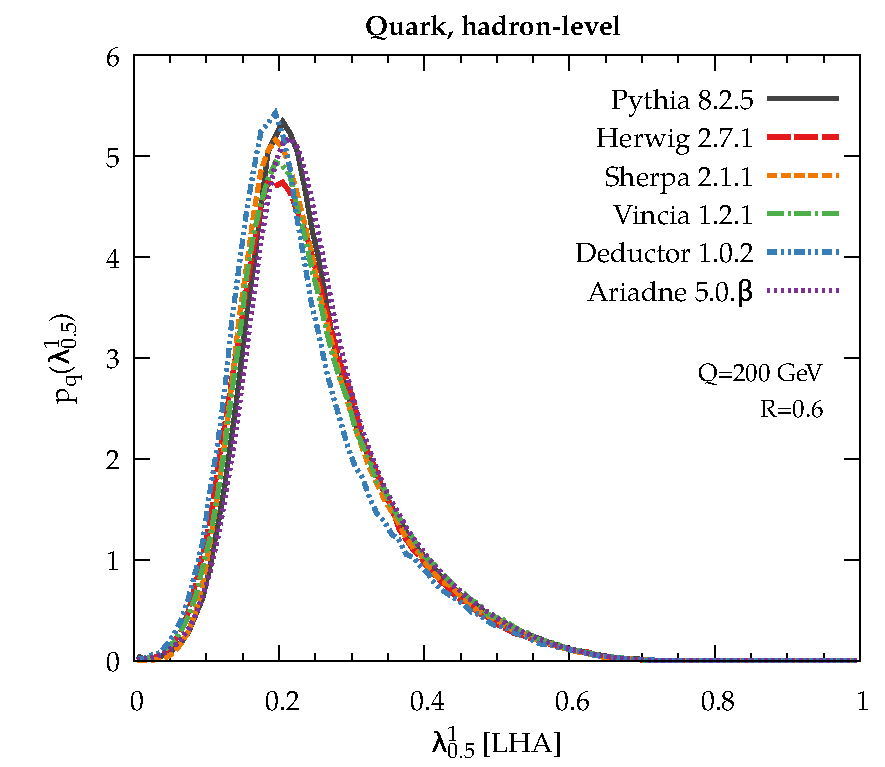
\includegraphics[width = 0.45\columnwidth]{quarkgluon_fig_GA_10_05_R6_hadron_quark.pdf}
\label{quarkgluon_fig:LHA_hadron_quark}
}
$\qquad$
\subfloat[]{
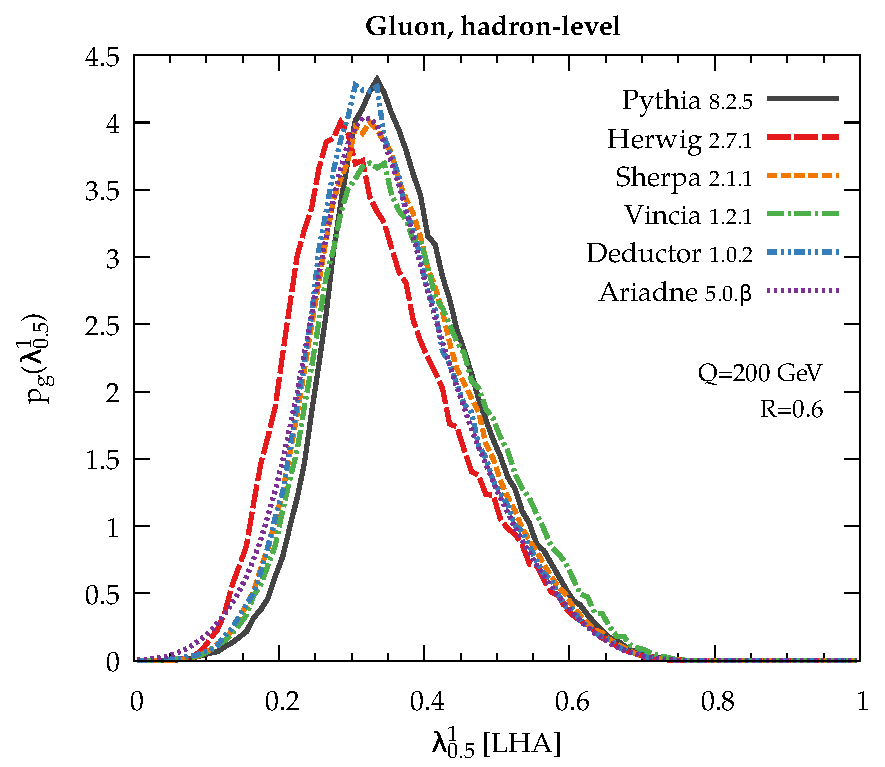
\includegraphics[width = 0.45\columnwidth]{quarkgluon_fig_GA_10_05_R6_hadron_gluon.pdf}
\label{quarkgluon_fig:LHA_hadron_gluon}
}

\subfloat[]{
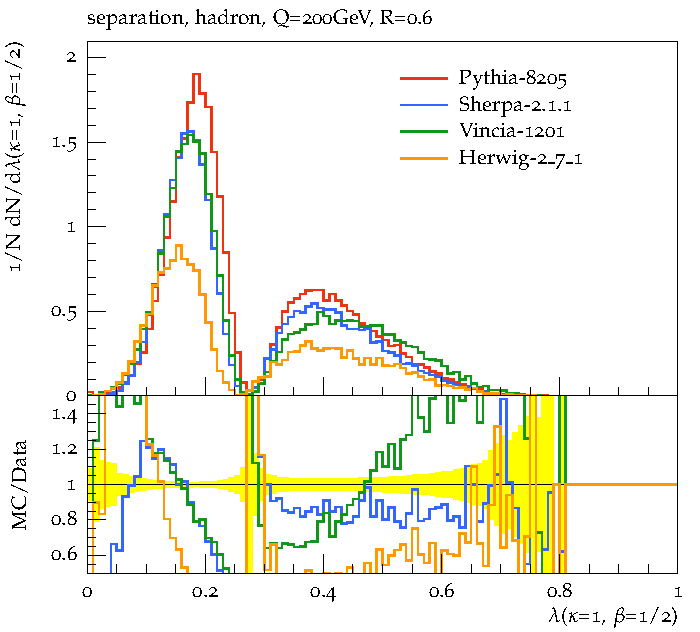
\includegraphics[width = 0.65\columnwidth]{quarkgluon_fig_GA_10_05_R6_hadron_separation.pdf}
\label{quarkgluon_fig:LHA_hadron_separation}
}
\caption{Hadron-level distributions of the LHA for (a) the $e^+ e^- \to u \bar{u}$ quark-tagged sample, (b) the $e^+ e^- \to gg$ gluon-tagged sample, and (c) the classifier separation integrand in Eq.~\eqref{quarkgluon_eq:deltaintegrand}.  All four parton shower generators---\textsc{Pythia 8.205}, \textsc{Vincia 1.201}, \textsc{Herwig++ 2.7.1}, \textsc{Sherpa 2.1.1}---are run at their baseline settings with center-of-mass energy $Q = 200~\GeV$ and jet radius $R= 0.6$.  \jdt{Is there a way to make the font size bigger in the yoda plots?  Need to say ratio to Pythia.}}
\label{quarkgluon_fig:LHA_hadron}
\end{figure}

In Fig.~\ref{quarkgluon_fig:LHA_hadron}, we show hadron-level distributions of the LHA (i.e.~$\lambda_{0.5}^1$) in the quark sample ($p_q$) and gluon sample ($p_g$), comparing the baseline settings of four different parton shower generators.  In the quark sample in Fig.~\ref{quarkgluon_fig:LHA_hadron_quark}, there is relatively little variation between the generators, which is not surprising since all four programs have been tuned to match LEP data (though LEP never measured the LHA itself).  Turning to the gluon sample in Fig.~\ref{quarkgluon_fig:LHA_hadron_gluon}, we see somewhat larger variations between the generators; this is expected since there is no data to directly constrain $e^+ e^- \to gg$.   We plot the integrand of classifier separation in Fig.~\ref{quarkgluon_fig:LHA_hadron_separation}:
\begin{equation}
\label{quarkgluon_eq:deltaintegrand}
\frac{1}{2} \frac{\bigl(p_q - p_g\bigr)^2}{p_q + p_g}.
\end{equation}
This quantity shows where in the LHA phase space the actual discrimination power lies, with large values of the integrand corresponding to places where the quark and gluon distributions are most dissimilar.  Now we see considerable differences between the generators, reproducing the well-known fact that \textsc{Pythia} is more optimistic about quark/gluon separation while \textsc{Herwig} is more pessimistic.  The prediction discrimination power from \textsc{Vincia} and \textsc{Sherpa} are intermediate between these extremes and similar to each other.

\begin{figure}
\centering
\subfloat[]{
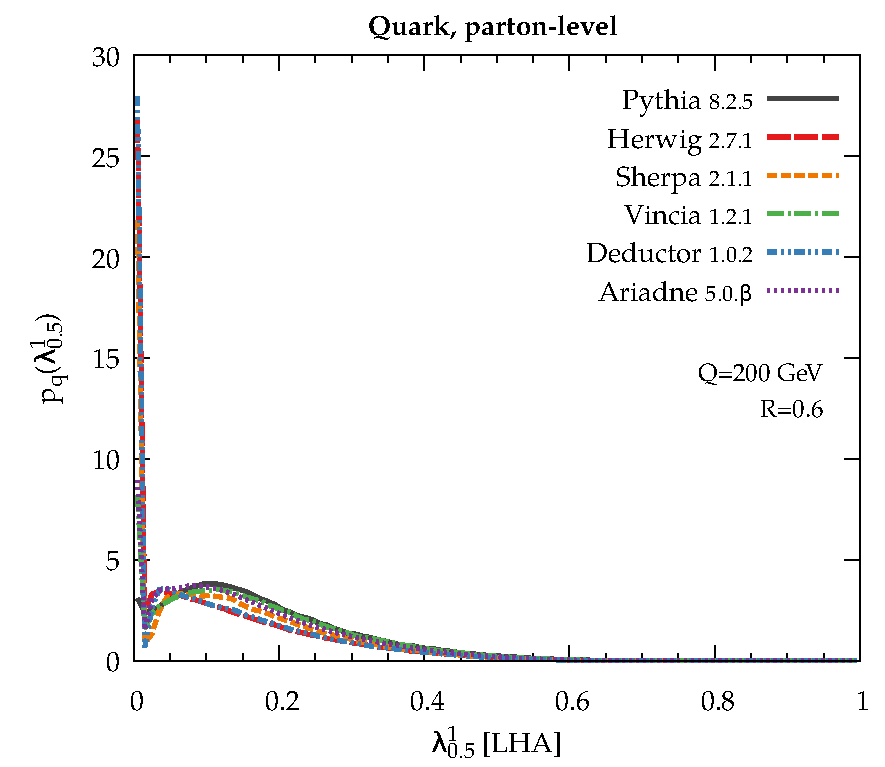
\includegraphics[width = 0.45\columnwidth]{quarkgluon_fig_GA_10_05_R6_parton_quark.pdf}
\label{quarkgluon_fig:LHA_parton_quark}
}
$\qquad$
\subfloat[]{
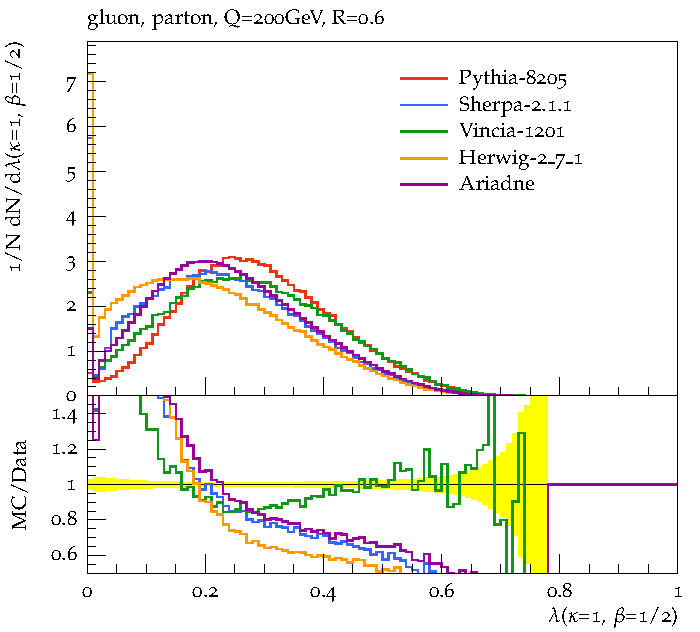
\includegraphics[width = 0.45\columnwidth]{quarkgluon_fig_GA_10_05_R6_parton_gluon.pdf}
\label{quarkgluon_fig:LHA_parton_gluon}
}

\subfloat[]{
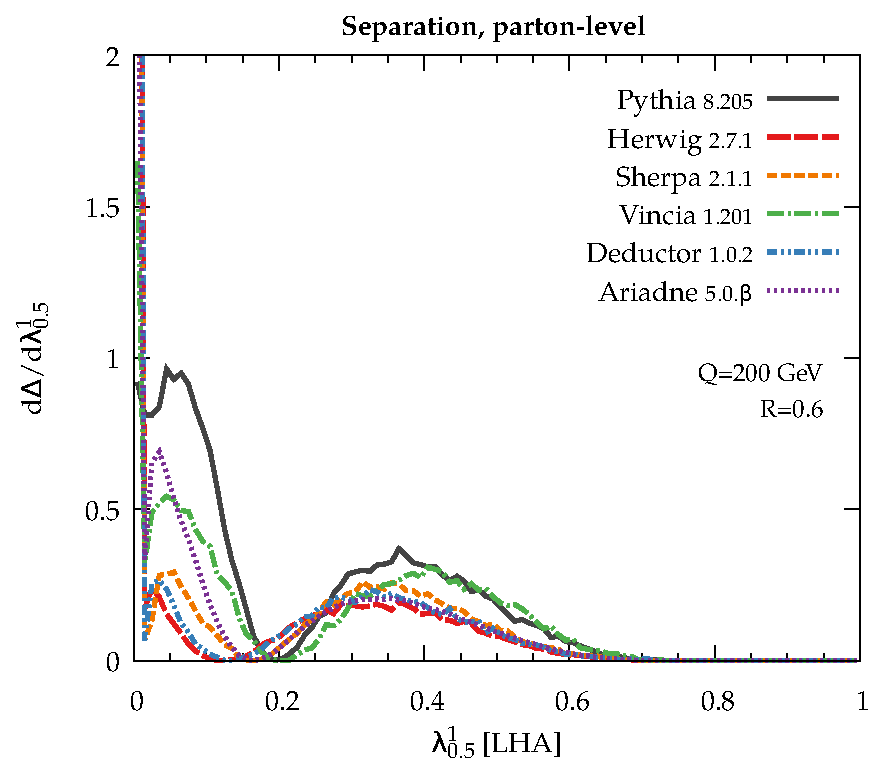
\includegraphics[width = 0.65\columnwidth]{quarkgluon_fig_GA_10_05_R6_parton_separation.pdf}
\label{quarkgluon_fig:LHA_parton_separation}
}
\caption{Same as Fig.~\ref{quarkgluon_fig:LHA_hadron}, but at the parton level.  Here, we have also included predictions from \textsc{Deductor 1.0.2}, which tend to agree with \textsc{Herwig++ 2.7.1}.}
\label{quarkgluon_fig:LHA_parton}
\end{figure}

One might expect that the differences between generators are due simply to their having different hadronization models.  It seems, however, that the differences already appear at the parton level prior to hadronization, as shown in Fig.~\ref{quarkgluon_fig:LHA_parton}.  The first thing one notices is that three of the generators---\textsc{Herwig}, \textsc{Sherpa}, and  \textsc{Deductor}---yield a large population of events where the perturbative shower generates no emissions, giving $\lambda_{0.5}^1 = 0$.  By contrast, \textsc{Pythia} and \textsc{Vincia} give overall larger values of the LHA from the perturbative shower alone.  Since Fig.~\ref{quarkgluon_fig:LHA_hadron_quark} shows that all generators give similar hadron-level distributions for quark jets after hadronization, we conclude that understanding quark/gluon discrimination is a challenge at the boundary between perturbative showering and non-perturbative hadronization.

\begin{figure}
\centering
\subfloat{
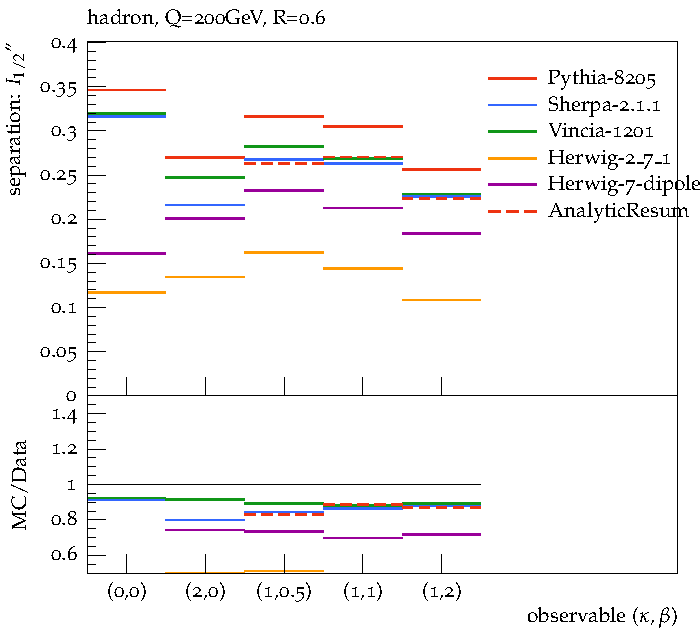
\includegraphics[width = 0.45\columnwidth]{quarkgluon_fig_I2_R6_hadron__all.pdf}
}
$\qquad$
\subfloat{
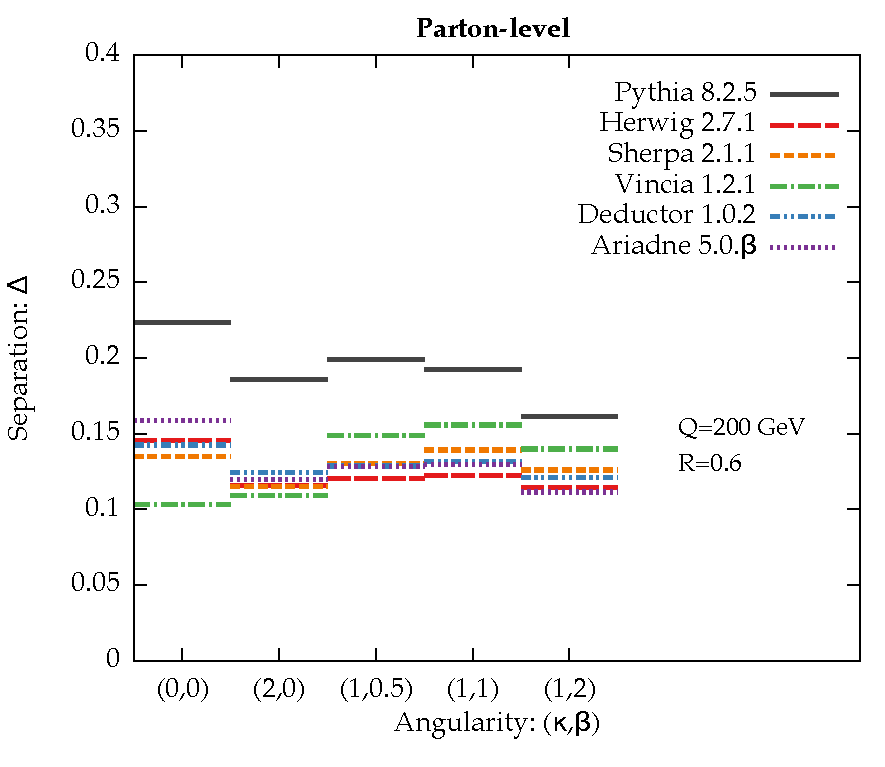
\includegraphics[width = 0.45\columnwidth]{quarkgluon_fig_I2_R6_parton__all.pdf}
}
\caption{Classifier separation $\Delta$ for the five different benchmark angularities in Eq.~\eqref{quarkgluon_eq:benchmarkang}, determined from the various generators at (a) hadron level and (b) parton level.  The first two columns correspond to IRC unsafe distributions (multiplicity and $p_T^D$), while the last three columns are the IRC safe angularities.  The LHA is shown in the middle column.}
\label{quarkgluon_fig:summary_hadron_all}
\end{figure}

To summarize the overall discrimination power, we integrate Eq.~\eqref{quarkgluon_eq:deltaintegrand} to obtain the value of $\Delta$ for the LHA.  This is shown in Fig.~\ref{quarkgluon_fig:summary_hadron_all}, which also includes the four other benchmark angularities from Eq.~\eqref{quarkgluon_eq:benchmarkang}.  There is a rather large spread in predicted discrimination power between the generators, especially at hadron level.  While such differences might be expected for IRC unsafe angularities (multiplicity and $p_T^D$) which depend on non-perturbative modeling, these differences persist even for the IRC safe angularities, indicating a more fundamental difference between the generators that is already present at parton level.

\subsection{Parameter Dependence}
\label{quarkgluon_sec:ee_scales}

\begin{figure}
\centering
\subfloat[]{
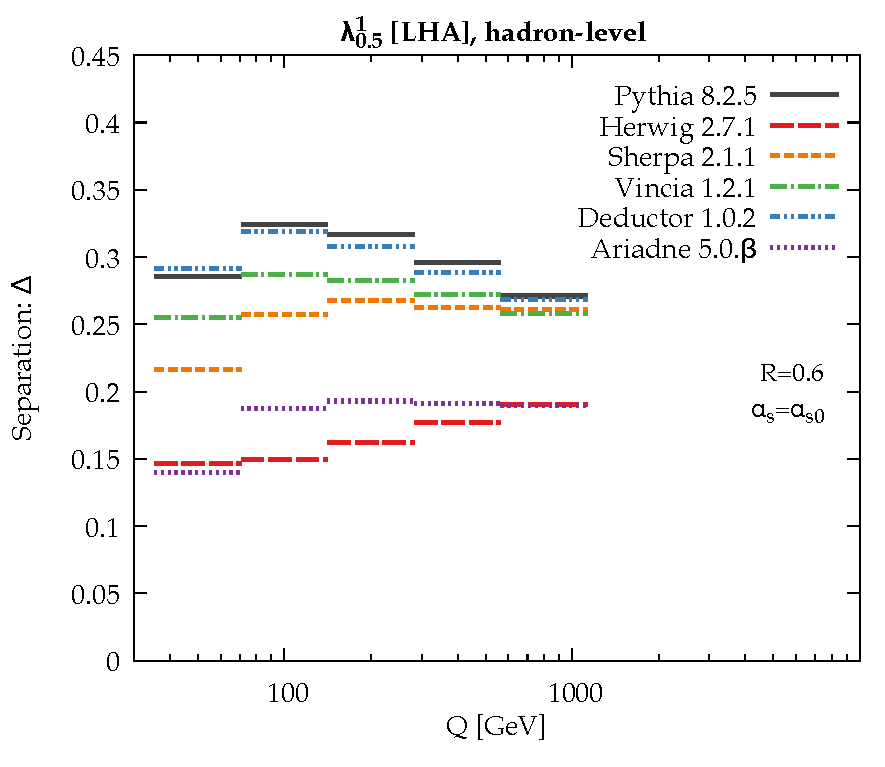
\includegraphics[width = 0.4\columnwidth]{quarkgluon_fig_I2_GA_10_05_hadron_Qdep.pdf}
\label{quarkgluon_fig:sweep_Q_hadron}
}
$\qquad$
\subfloat[]{
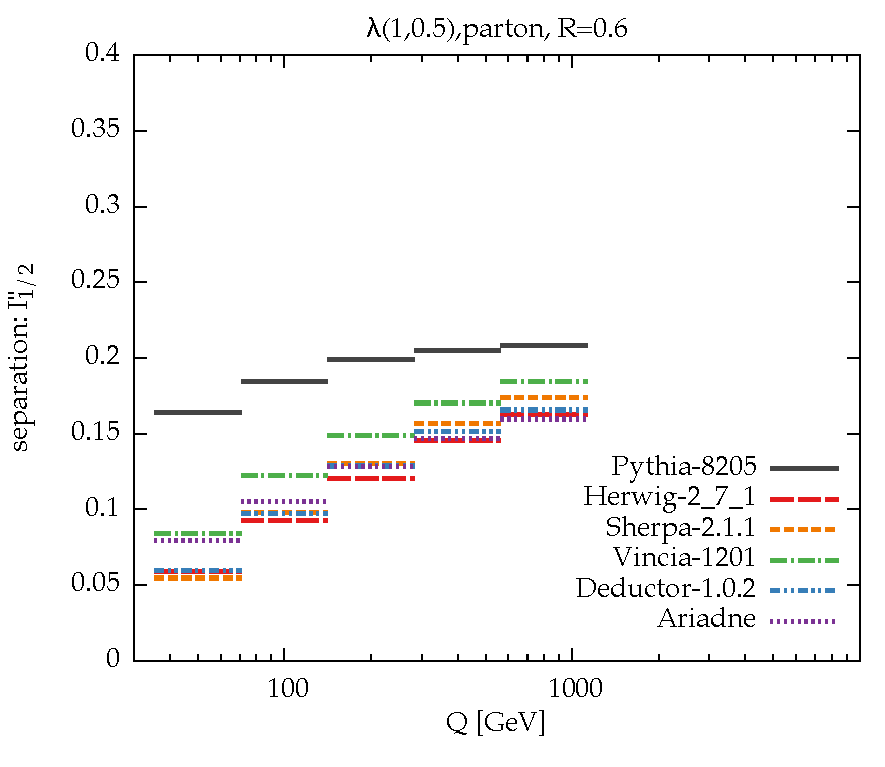
\includegraphics[width = 0.4\columnwidth]{quarkgluon_fig_I2_GA_10_05_parton_Qdep.pdf}
\label{quarkgluon_fig:sweep_Q_parton}
}

\subfloat[]{
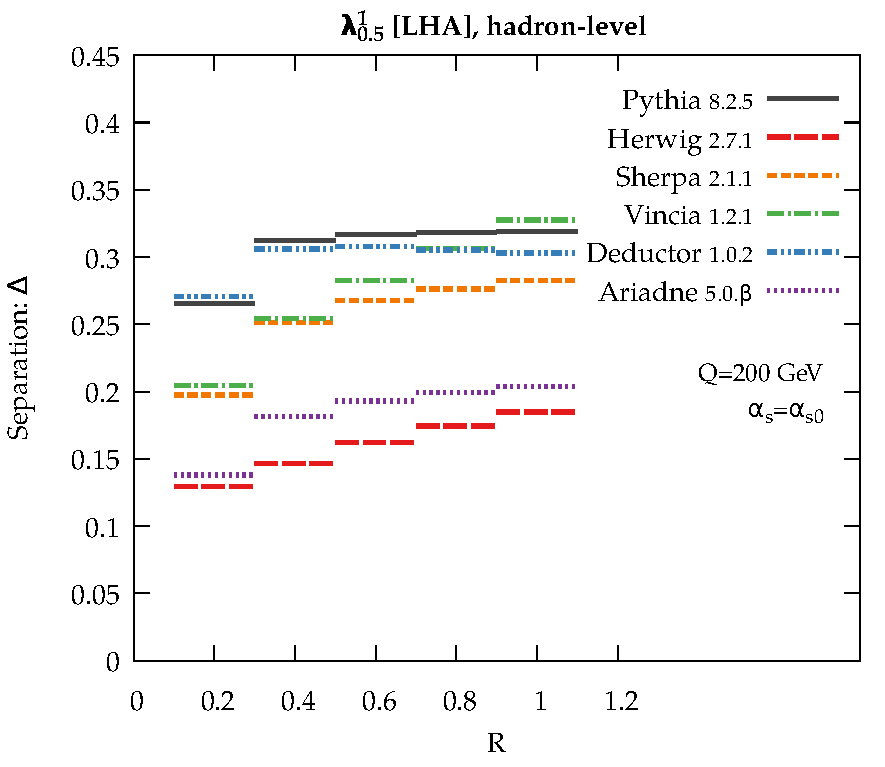
\includegraphics[width = 0.4\columnwidth]{quarkgluon_fig_I2_GA_10_05_hadron_Rdep.pdf}
\label{quarkgluon_fig:sweep_R_hadron}
}
$\qquad$
\subfloat[]{
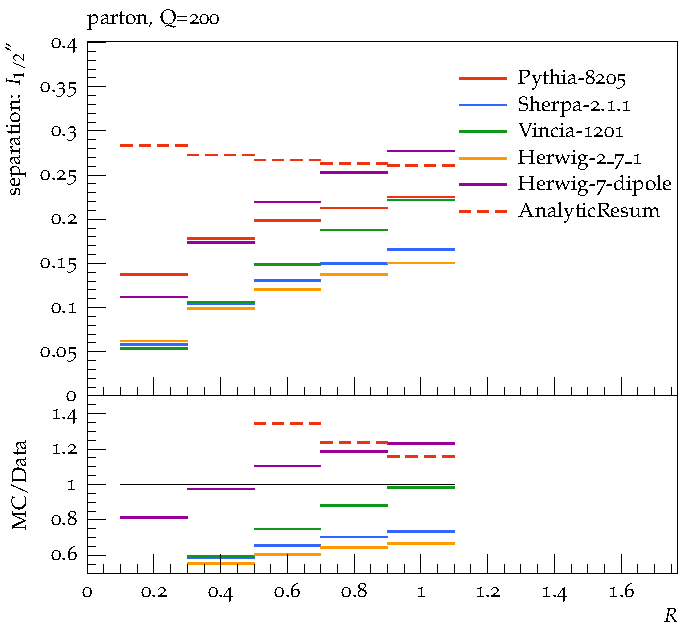
\includegraphics[width = 0.4\columnwidth]{quarkgluon_fig_I2_GA_10_05_parton_Rdep.pdf}
\label{quarkgluon_fig:sweep_R_parton}
}

\subfloat[]{
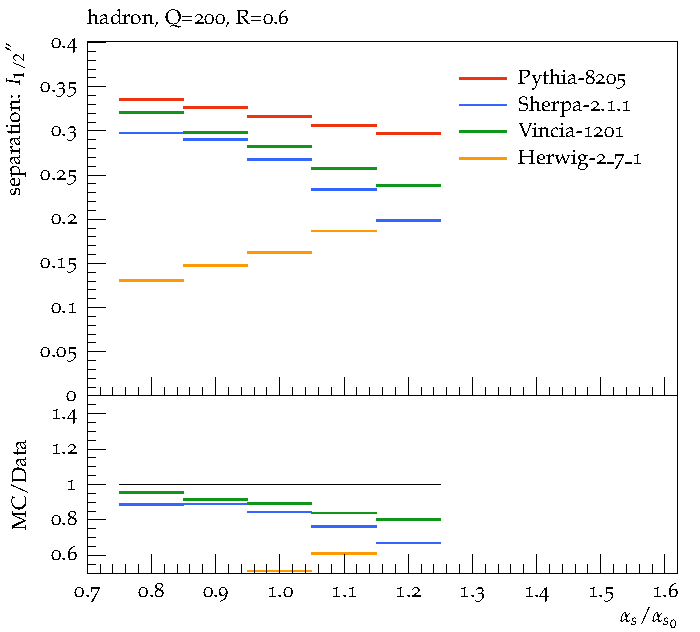
\includegraphics[width = 0.4\columnwidth]{quarkgluon_fig_I2_GA_10_05_hadron_alphadep.pdf}
\label{quarkgluon_fig:sweep_as_hadron}
}
$\qquad$
\subfloat[]{
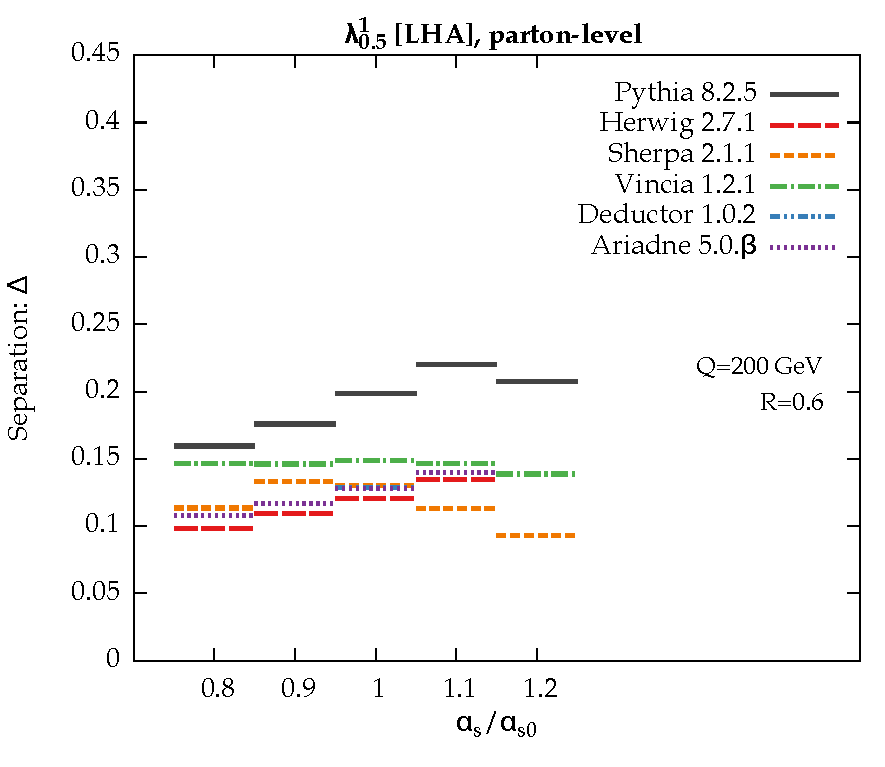
\includegraphics[width = 0.4\columnwidth]{quarkgluon_fig_I2_GA_10_05_parton_alphadep.pdf}
\label{quarkgluon_fig:sweep_as_parton}
}
\caption{Classifier separation $\Delta$ for the LHA, sweeping the collision energy $Q$ (top row), jet radius $R$ (middle row), and coupling constant $\alpha_s/\alpha_{s0}$ (bottom row).  Results are shown at hadron level (left column) and at the parton level (right column).  \jdt{We need to label the plots as saying that they are for the LHA.}}
\label{quarkgluon_fig:ee_sweep}
\end{figure}

Given the large absolute differences in discrimination power seen above, we next want to check if the parton shower generators exhibit similar or dissimilar trends as parameters are varied.  We perform three parameter sweeps, using the bolded values below as defaults:
\begin{equation}
\begin{aligned}
\text{Collision Energy}: Q &= \{ 50, 100, \mathbf{200}, 400, 800\}~\GeV, \\
\text{Jet Radius}: R &= \{ 0.2, 0.4, \mathbf{0.6}, 0.8, 1.0\}, \\
\text{Strong Coupling}: \alpha_s / \alpha_{s0} &= \{0.8,0.9,\mathbf{1.0},1.1,1.2\}, \\
\end{aligned}
\end{equation}
where $\alpha_{s0}$ is the default value of the coupling, which is different between the generators (and sometimes different between different aspects of the same generator).

The resulting values of $\Delta$ are shown in Fig.~\ref{quarkgluon_fig:ee_sweep}, at both the hadron level and parton level.   There are number of surprising features in these plots.  First, even for the IRC safe angularities, the effect of hadronization is rather large, both on the absolute scale of discrimination and the trends.  The main exception to that trend is \textsc{Herwig}, which does not exhibit much of an effect from hadronization.  Second, the trends for sweeping $Q$ and sweeping $\alpha_s$  seem contradictory.  According to the perturbative logic in ref.~\cite{Larkoski:2013eya} at next-to-leading-logarithmic (NLL) accuracy, larger values of $\alpha_s$ should lead to improved discrimination power (which is seen for \textsc{Herwig} but not the other generators).  But larger values of $Q$ correspond to smaller values of $\alpha_s$, so increasing $Q$ was expected to lead to worse discrimination power (seen by none of the generators at parton level, and somewhat present for all the generators \emph{except} \textsc{Herwig} at hadron level).  Third, the trend for sweeping $R$ is again backwards from the logic in ref.~\cite{Larkoski:2013eya}, where larger jet radii were expected to yield worse separation power (seen by none of the generators).

We suspect that part of the issue is that ref.~\cite{Larkoski:2013eya} did not include non-perturbative hadronization corrections, which could potentially reverse the perturbative trends.  That said, some of these confusions are present already at parton level, so further study is needed to test whether additional perturbative effects beyond NLL could explain these features.  At NLL accuracy, one accounts for the fact that a jet can contain multiple perturbative emissions, but those emissions are treated as if they themselves do not radiate.  Therefore, the fact that parton showers allow every emission to reradiate might explain these surprising quark/gluon discrimination trends.

\subsection{Impact of Generator Settings}
\label{quarkgluon_sec:ee_settings}

Formally, parton shower generators are only accurate to modified leading logarithmic (MLL) accuracy, though they usually include physically important effects like energy/momentum conservation and matrix element corrections that go beyond MLL.  We can assess the impact of these higher-order effects by changing the baseline parameter settings in each of the generators.  

Because each generator is different, we cannot always make the same changes for each generator.  Similarly, the spread in discrimination power shown below should \emph{not} be seen as representing the intrinsic uncertainties in the shower, since many of these changes are not physically motivated.  The goal of these plots is to demonstrate possible areas where small parameter changes could have a large impact on quark/gluon discrimination.  Ultimately, collider data and higher-order calculations will be essential for understanding the origin of quark/gluon differences.  In all cases, we show both hadron-level and parton-level results, even if a setting is only expected to have an impact at the hadron level.  


In the top row of Fig.~\ref{quarkgluon_fig:settings_variation_pythia}, we consider the following variations for  \textsc{Pythia}:  \jdt{We should probably give these nicer names}
\begin{itemize}
\item \textsc{Pythia-CR1}.  Often, one thinks of color reconnection as being primarily important for hadron colliders, but even at a lepton collider, color reconnection will change the QCD strings used for hadronization.  This variation uses an alternative color reconnection model compared to the default \jdt{Is is alternative or just off?}.  At parton level, this variation has no effect as expected.  At hadron level, this variation considerably decreases quark/gluon separation compared to the baseline.
\item \textsc{Pythia-CR2}.  \jdt{This variation seems to not be useful, right?}
\item \textsc{Pythia-a2L}.  The default \textsc{Pythia} setting is to use 1-loop running for $\alpha_s$.  This variation turns on 2-loop running for $\alpha_s$, which has a small (beneficial) effect at parton level which is washed out at hadron level.
\item \textsc{Pythia-nogqq}.  The dominant gluon splitting in the parton shower is $g \to gg$, but there are also $g \to q \bar{q}$ splittings present in \textsc{Pythia}.  This variation turns off $g \to q \bar{q}$, which makes gluon jets look more gluon-like, thereby increasing the separation power.
\item \textsc{Pythia-nome}.  The first emission in \textsc{Pythia} improved by imposing a matrix element correction.  This correction has relatively little effect on our studies, though, since there is no matrix element available for $h^* \to g g$.
\item \textsc{Pythia-norec}.  \jdt{This setting seems to not be useful, right?}
\end{itemize}
The most surprising \textsc{Pythia} effect is related to color reconnection, which will also turn out to be important for the \textsc{Herwig} generator below.

In the bottom row of Fig.~\ref{quarkgluon_fig:settings_variation_vincia}, we consider the following variations for  \textsc{Vincia}:
\begin{itemize}
\item \textsc{Vincia-a2L}.
\item \textsc{Vincia-muq}.
\item \textsc{Vincia-nome}.
\item \textsc{Vincia-nogqq}.
\item \textsc{Vincia-norec}.
\end{itemize}

In the top row of Fig.~\ref{quarkgluon_fig:settings_variation_herwig}, we consider the following variations for  \textsc{Herwig}:
\begin{itemize}
\item \textsc{Herwig-dipole}.
\item \textsc{Herwig-dipoleNoCR}.
\item \textsc{Herwig-nocr}.
\item \textsc{Herwig-nogqq}.
\end{itemize}

Finally, in the bottom row of Fig.~\ref{quarkgluon_fig:settings_variation_sherpa}, we consider the following variations for \textsc{Sherpa}:
\begin{itemize}
\item \textsc{Sherpa-njet0}.
\item \textsc{Sherpa-njet1}.
\item \textsc{Sherpa-noqq}.
\end{itemize}


\begin{figure}
\centering
\subfloat[]{
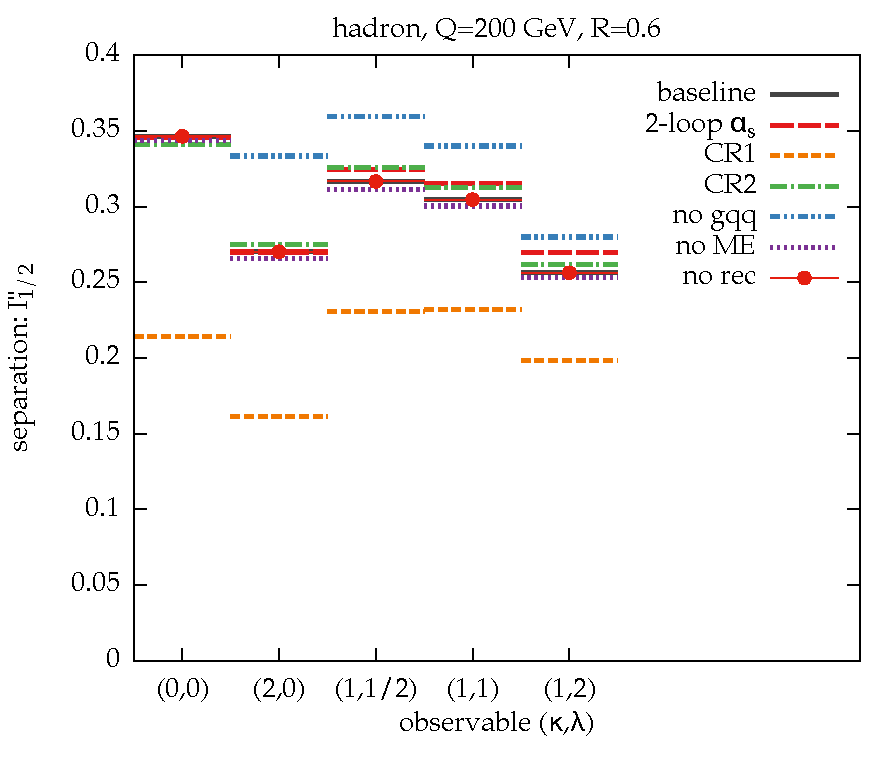
\includegraphics[width = 0.45\columnwidth]{quarkgluon_fig_I2_R6_hadron_pythia.pdf}
\label{quarkgluon_fig:summary_hadron_pythia}
}
$\qquad$
\subfloat[]{
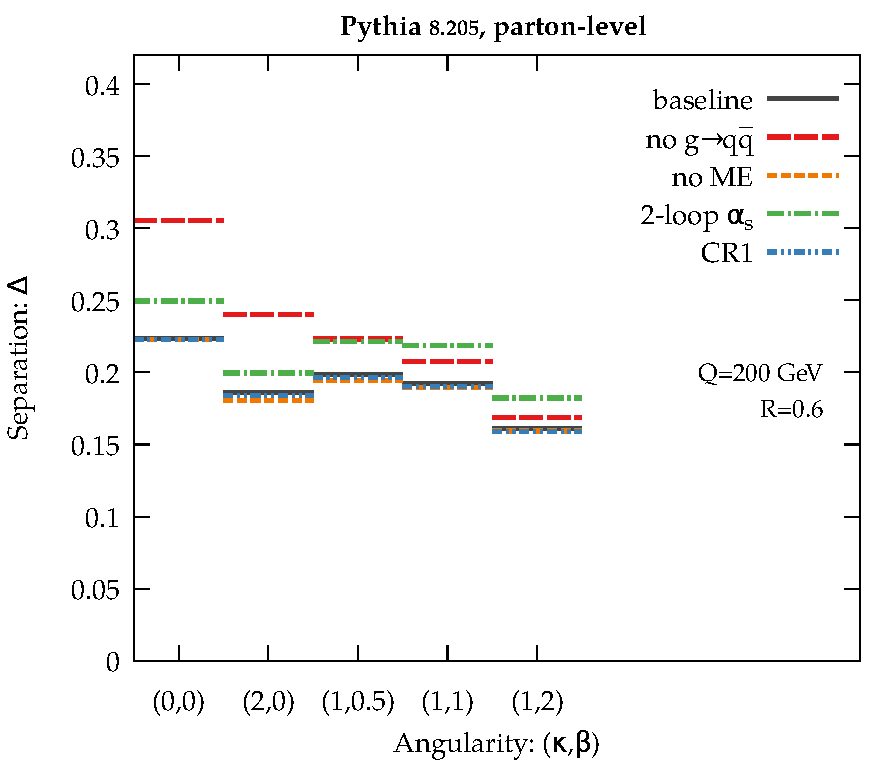
\includegraphics[width = 0.45\columnwidth]{quarkgluon_fig_I2_R6_parton_pythia.pdf}
\label{quarkgluon_fig:summary_parton_pythia}
}
\caption{Settings variants in \textsc{Pythia 8.205}.  Shown are hadron-level results (left column) and parton-level results (right column) for the classifier separation $\Delta$ for the LHA.}
\label{quarkgluon_fig:settings_variation_pythia}
\end{figure}


\begin{figure}
\centering
\subfloat[]{
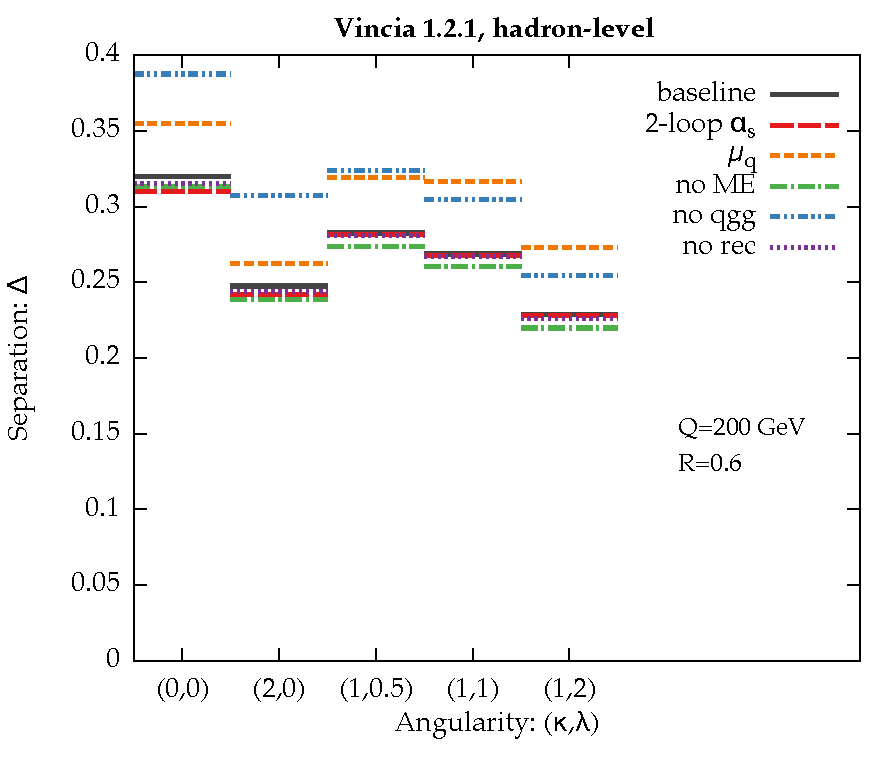
\includegraphics[width = 0.45\columnwidth]{quarkgluon_fig_I2_R6_hadron_vincia.pdf}
\label{quarkgluon_fig:summary_hadron_vincia}
}
$\qquad$
\subfloat[]{
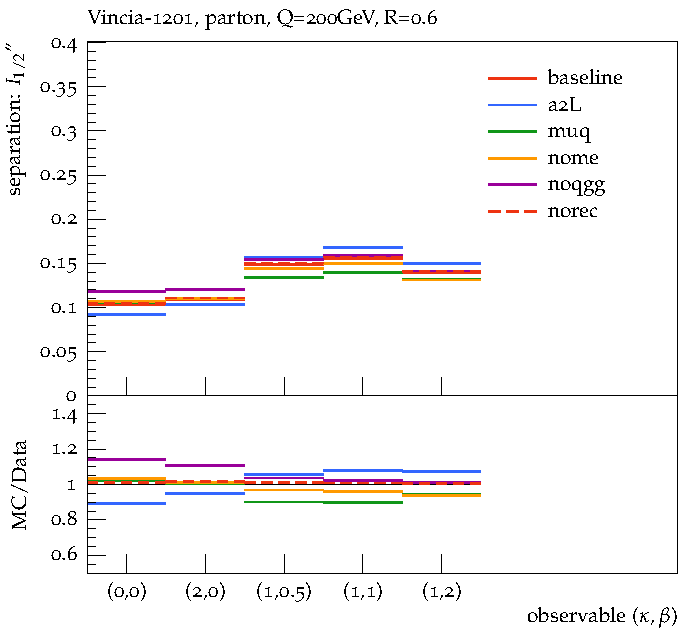
\includegraphics[width = 0.45\columnwidth]{quarkgluon_fig_I2_R6_parton_vincia.pdf}
\label{quarkgluon_fig:summary_parton_vincia}
}
\caption{Same as Fig.~\ref{quarkgluon_fig:settings_variation_pythia}, but for \textsc{Vincia 1.201}.}
\label{quarkgluon_fig:settings_variation_vincia}
\end{figure}

\begin{figure}
\centering
\subfloat[]{
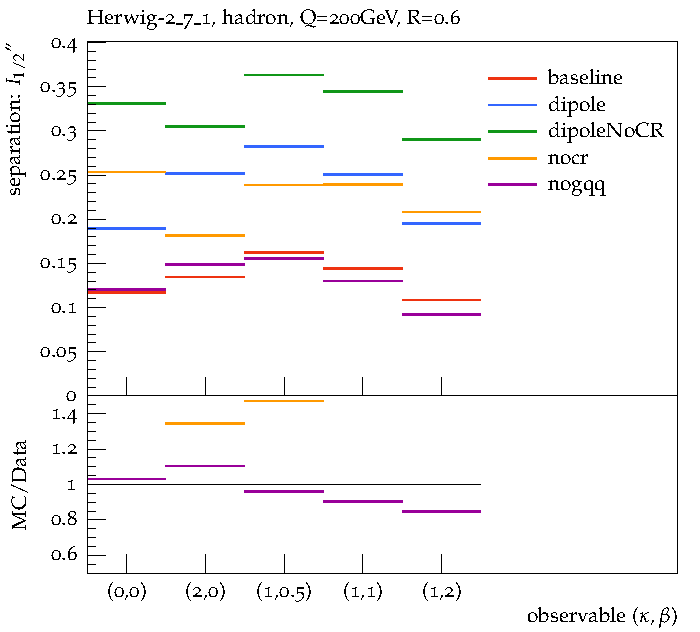
\includegraphics[width = 0.45\columnwidth]{quarkgluon_fig_I2_R6_hadron_herwig.pdf}
\label{quarkgluon_fig:summary_hadron_herwig}
}
$\qquad$
\subfloat[]{
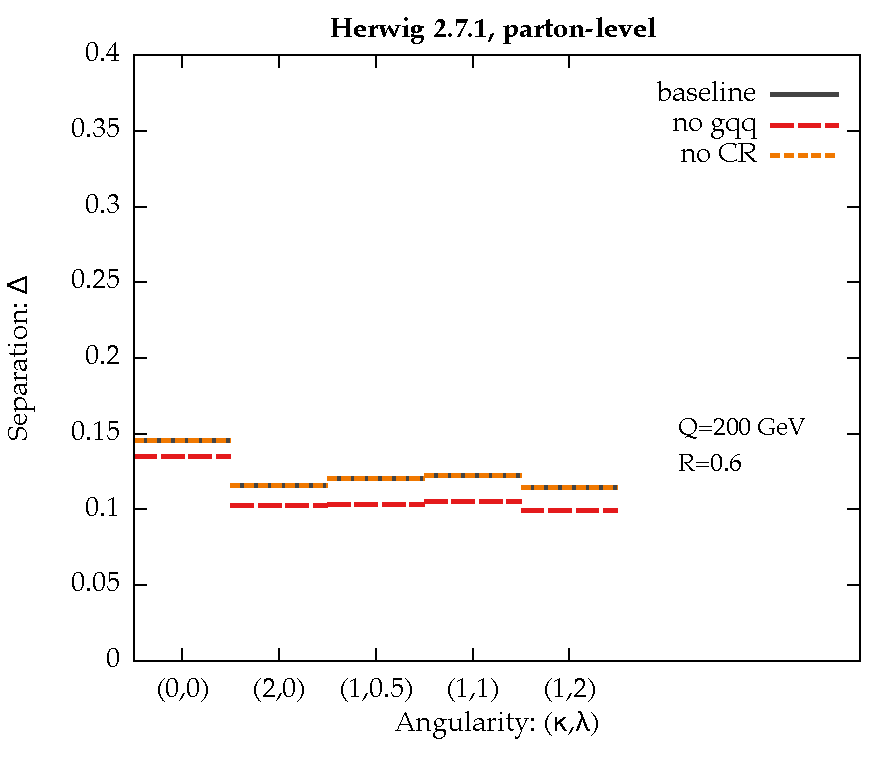
\includegraphics[width = 0.45\columnwidth]{quarkgluon_fig_I2_R6_parton_herwig.pdf}
\label{quarkgluon_fig:summary_parton_herwig}
}
\caption{Same as Fig.~\ref{quarkgluon_fig:settings_variation_pythia}, but for \textsc{Herwig 2.7.1}.  \jdt{We are missing some Herwig parton level.}}
\label{quarkgluon_fig:settings_variation_herwig}
\end{figure}

\begin{figure}
\centering
\subfloat[]{
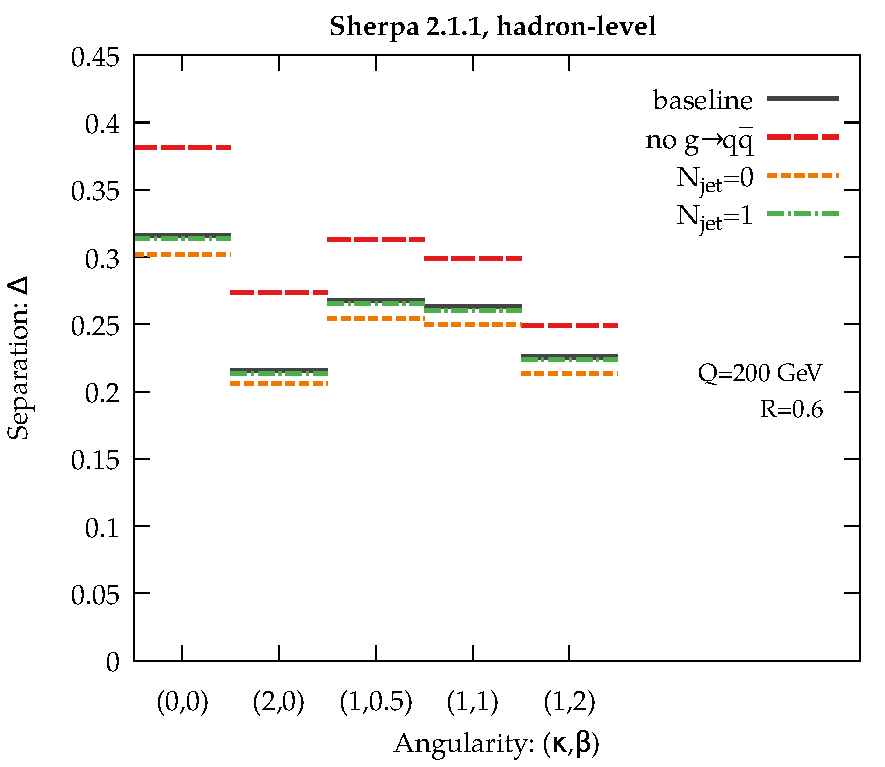
\includegraphics[width = 0.45\columnwidth]{quarkgluon_fig_I2_R6_hadron_sherpa.pdf}
\label{quarkgluon_fig:summary_hadron_sherpa}
}
$\qquad$
\subfloat[]{
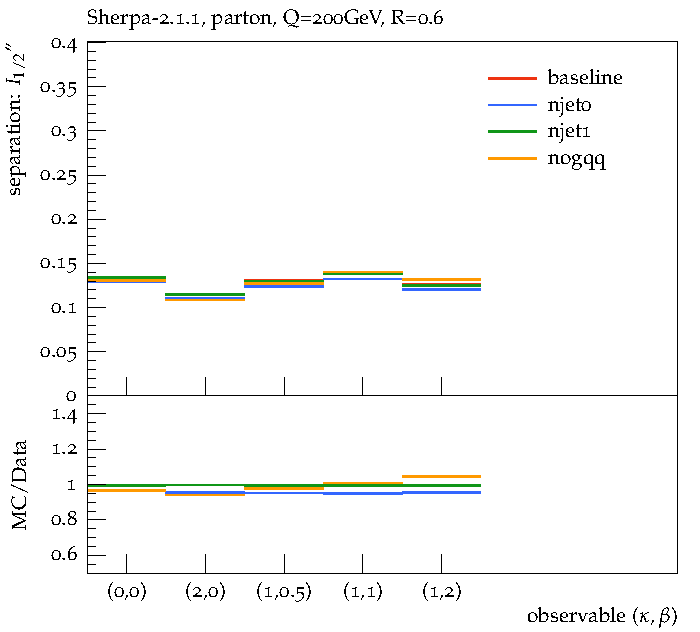
\includegraphics[width = 0.45\columnwidth]{quarkgluon_fig_I2_R6_parton_sherpa.pdf}
\label{quarkgluon_fig:summary_parton_sherpa}
}
\caption{Same as Fig.~\ref{quarkgluon_fig:settings_variation_pythia}, but for \textsc{Sherpa 2.1.1}. \jdt{Confused about the naming for Sherpa at parton level and hadron level.}}
\label{quarkgluon_fig:settings_variation_sherpa}
\end{figure}

\subsection{Looking Towards the LHC}
\label{quarkgluon_sec:pp}

It is clear from our $e^+e^-$ study that quark/gluon radiation patterns are not under good theoretical control, even accounting only for final state physics effects.  Beyond just the application to quark/gluon tagging, this is an important challenge for any analysis that uses jets.  In order to resolve these issues and improve parton shower modeling of jets, measurements from the LHC will be essential (as will improved analytic calculations).  In this section, we perform an example analysis for $pp$ collisions that highlights the kind of information one can gain about quark/gluon radiation patterns, despite the additional complications faced by hadronic collisions.

\begin{figure}
\centering
\subfloat{
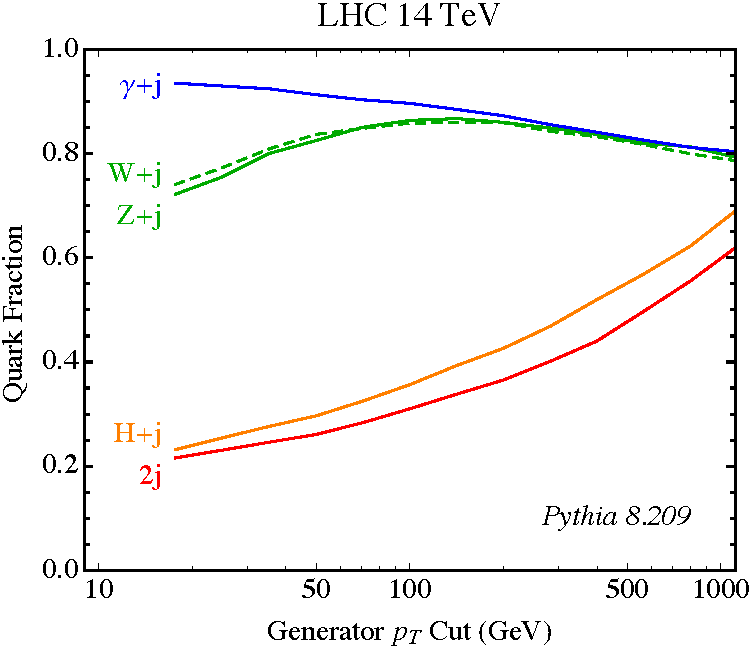
\includegraphics[width = 0.45\columnwidth]{quarkgluon_fig_parton_level_qg_composition.pdf}
}
\caption{Quark fraction of jets at parton level, as defined by the generator-level parton flavor.}
\label{quarkgluon_fig:parton_level_qg_composition}
\end{figure}

There is no way to isolate pure samples of quark or gluon jets at the LHC, but we can isolate quark/gluon-enriched samples, as defined by the flavor label of the jet in the corresponding Born-level partonic process.  As shown in Fig.~\ref{quarkgluon_fig:parton_level_qg_composition}, the Born-level jet in $W/Z/\gamma + \text{jet}$ is more than 70\% quark enriched over the entire jet $p_T$ range of interest.  For jets softer than around 200 GeV, the Born-level jet in dijets or $H+\text{jet}$ is more than 60\% gluon enriched, with that fraction decreasing as the jet $p_T$ increases.  In principle, could could try to ``diagonalize" some combination of vector boson plus jet and dijet samples in order to define separate quark or gluon samples (see \cite{}).  In this study, we will simply ask the question whether one can tell ``the jets in $Z$ plus jet" (quark-enriched) apart from "the jets in dijets" (gluon-enriched).  

In Fig.~\ref{quarkgluon_}, we show LHA distributions for quark-enriched and gluon-enriched samples.  \jdt{Need plot to say more.}

\subsection{Summary and Recommendations}
\label{quarkgluon_sec:conclude}

By measuring the substructure of jets, it is possible to gain information about the quark/gluon composition of a jet sample.  The challenge we have identified in this paper is that the precise radiation pattern of quark and gluon jets is poorly understood, in the sense that parton shower generators give rather different predictions for absolute quark/gluon discrimination power as well as relative trends as a function of the jet kinematics.  At the moment, analytic calculations are not at a level of accuracy where they can offer any useful guide.  Therefore, LHC data is the best hope to constrain quark/gluon radiation patterns and enable quark/gluon discrimination to be a robust tool.

In terms of specific measurements that should be highest priority for ATLAS and CMS, our study has not revealed a silver bullet.  \jdt{Still true in pp with grooming?}  Rather, all of the generalized angularities studies showed similar levels of disagreement between generators, so a systematic LHC study of even one observable is likely to offer crucial new information.  What is essential is to make measurements at multiple jet $p_T$ scales and multiple jet radii $R$.  Unfolded distributions would likely be most useful for parton shower tuning, but even detector-level measurements compared to detector-simulated parton showers would help spot troubling trends.

The key lesson to parton shower authors is that LEP data \emph{does not} constrain all of the relevant aspects of the final state parton shower.  While we have extensive information about quark jet radiation patterns, gluon jet radiation patterns are essentially unconstrained.  This has important implications for parton shower tuning strategies.  Specific recommendations:
\begin{itemize}
\item \textit{Gluon splitting to quarks}:  Some of the largest difference between generators came from turning on and off the $g \to q \overline{q}$ process.  \jdt{...}
\item \textit{Color reconnection in the final state}:  Color reconnection is usually thought of as an issue mainly at hadron colliders.  \jdt{...}
\item \textit{Reconsidering $\alpha_s$ defaults}:  \jdt{...}
\end{itemize}


\bibliography{quarkgluon_bib}

\end{document}
